\section{Scelta del modello}
Si riportano i valori di $R^2$ e AIC dei quattro modelli.
\begin{table}[H]
	\centering
	\begin{tabular}{|c|c|c|}
		\hline
		\textbf{Modello} & \textbf{adjusted} \boldmath$R^2$ & \textbf{AIC} \\
		\hline
		1 &  0.77  & 514.69 \\
		2 & 0.87 & 460.76 \\
		3 & 0.77 & 514.11 \\
		4 & 0.89 & 448.27 \\
		\hline
	\end{tabular}
	\caption{Valori di $R^2$ e AIC per i quattro modelli}
\end{table}
Di seguito vengono mostrati i grafici diagnostici ottenuti sui quattro modelli.
\begin{figure}[H]
	\centering
	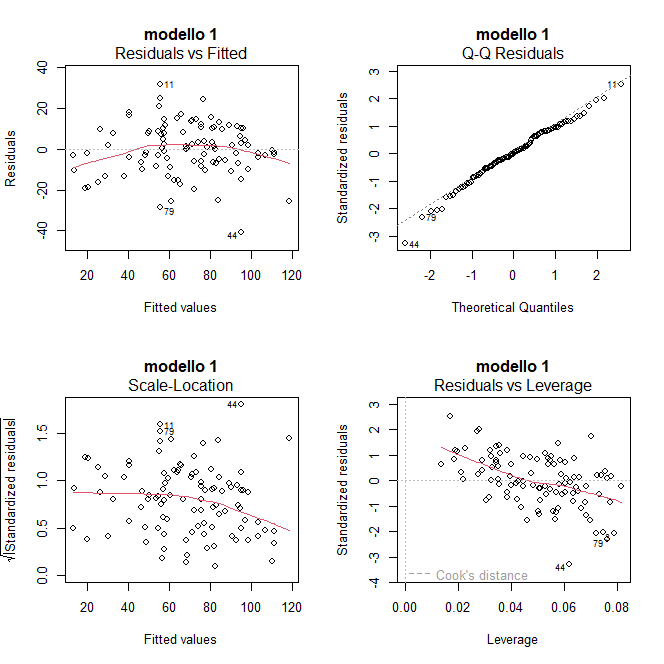
\includegraphics[width=1\linewidth]{../graphs/diagnostica/diagnostica_ridotto}

	\label{fig:diagnosticaridotto}
\end{figure}
\begin{figure}[H]
	\centering
	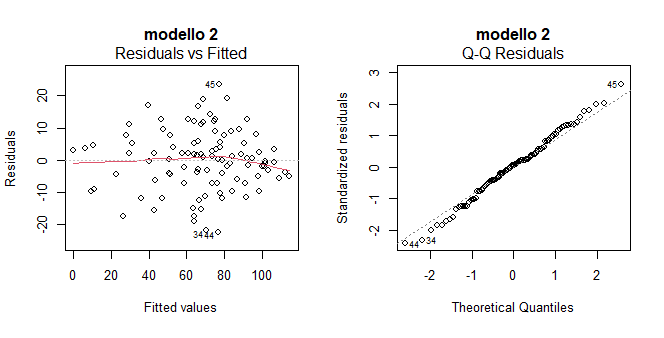
\includegraphics[width=1\linewidth]{../graphs/diagnostica/diagnostica_quadrato}

	\label{fig:diagnosticaridotto}
\end{figure}
\begin{figure}[H]
	\centering
	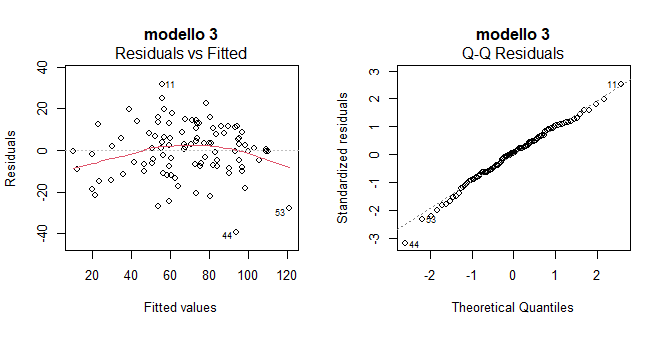
\includegraphics[width=1\linewidth]{../graphs/diagnostica/diagnostica_stepwise}

	\label{fig:diagnosticaridotto}
\end{figure}
\begin{figure}[H]
	\centering
	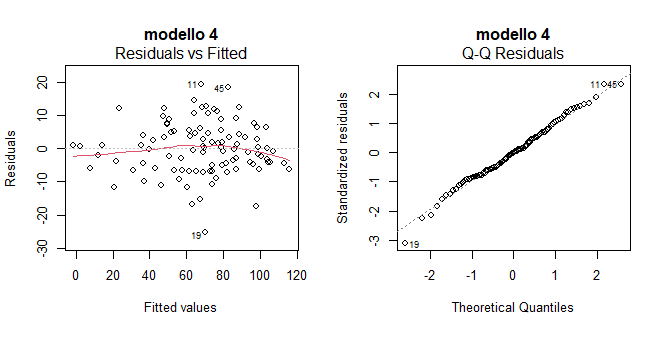
\includegraphics[width=1\linewidth]{../graphs/diagnostica/diagnostica_stepwise_iterations}
	\label{fig:diagnosticaridotto}
	\caption{Residuals vs Fitted e Q-Q Residuals dei quattro modelli.}
\end{figure}
Osservando i grafici 


